%%%%%%%%%%%%%%%%%%%%%%%%%%%%%%%%%%%%%%%%%%%%%%%%%%%
% LaTeX model for Rougemont chapters and articles %
%%%%%%%%%%%%%%%%%%%%%%%%%%%%%%%%%%%%%%%%%%%%%%%%%%%
% Needed before document class
\RequirePackage{pdftexcmds} % needed for tests expressions
\RequirePackage{fix-cm} % correct units

\documentclass[twocolumn]{article}
\usepackage[%
  a4paper,
  inner=15mm,
  outer=15mm,
  top=20mm,
  bottom=18mm,
  marginparsep=0pt,
]{geometry}
\setlength{\columnsep}{10mm}

%% Teinte
\input{vendor/oeuvres/xsl/tei_latex/teinte}

\directlua{luaotfload.add_fallback
   ("mathfallback", {
      % https://learn.microsoft.com/en-us/typography/opentype/spec/scripttags
      "DejaVuSans:mode=harf;" % ;script=math
    })
}

\setmainfont[
    UprightFont    = SourceSans3-Light,
    ItalicFont     = SourceSans3-LightIt,
    BoldFont       = SourceSans3-Semibold,
    BoldItalicFont = SourceSans3-SemiboldIt,
    Renderer=HarfBuzz,
    RawFeature={fallback=mathfallback},
]{Source Sans 3 Light}


% document language
\usepackage[french]{babel}
\selectlanguage{french}


\renewcommand{\headrulewidth}{0.1pt}
\renewcommand{\headrule}{{\color{rubric}\hrule}}
\renewcommand{\thefootnote}{\bfseries\textcolor{rubric}{\arabic{footnote}}} % color for footnote marks
\titleformat{name=\section}
  [display]{}{}{}{}
  [\RaggedRight\setstretch{0.95}\color{rubric}\Large\textbf{#1}]
% \titlespacing{\section}{0pt}{0pt plus 4pt minus 2pt}{\baselineskip}

\fancypagestyle{main}{%
  \fancyhf{}
  \setlength{\headheight}{1.5em}
  \fancyhead{} % reset head
  \fancyfoot{} % reset foot
  \fancyhead[L]{\truncate{0.45\headwidth}{\fontrun\elbibl}} % book ref
  \fancyhead[R]{\truncate{0.45\headwidth}{ \fontrun\nouppercase\eltitle}} % Chapter title
  \fancyhead[C]{\thepage}
}

\renewenvironment{quoteblock}
  {\begin{quoting}\smaller} %
  {\end{quoting}}


\begin{document}

\thispagestyle{empty}
\twocolumn[{%
  \begin{tikzpicture}[remember picture,overlay]
    \node[xshift=15mm,yshift=-15mm,anchor=north west] at (current page.north west){%
      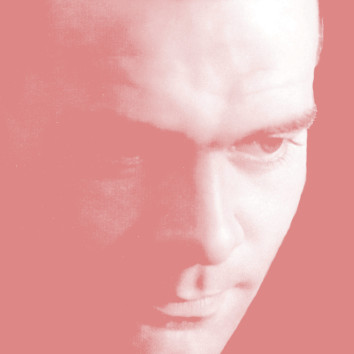
\includegraphics[width=30mm]{ddr-red.jpg}
    };
    \node[xshift=15mm,yshift=-6mm,anchor=north west] at (current page.north west){%
      
\includegraphics[width=50mm]{rougemont20-noir.png}
    };
  \end{tikzpicture}
  \vskip-2em
  \setlength{\RaggedLeftLeftskip}{33mm plus 1em} % plus is needed, don’t ask why
  \RaggedLeft\parindent0pt
  \LARGE\elauthor (\eldate)\par
  \Large\normalfont \emph{\elbook}\par
  \href{\elurl}{\eltitle}\footnotemark\par
  \vskip3em
}]
\footnotetext{\href{\elurl}{\elurl}}
\pagestyle{main} % after style
\bigskip
\makeatletter\@starttoc{toc}\makeatother % toc without new page
\bigskip



%text%


\end{document}
